\documentclass[11pt,letterpaper]{article}
\usepackage{psfrag,graphicx,epsfig}
\usepackage{amsmath,amsfonts,amssymb,amsthm}


\begin{document}

%% Simulation Block Diagram
 %%%%%%%%%%%%%%%%%%%%%%%%

\begin{center}
 \section*{Simulation Block Diagram Reduction}
\end{center}

\begin{figure}[htb]
 \centering
 \includegraphics{./final_figures/linear_sim_s_domain}
 \caption{Linear Model Block Diagram}
 \label{fig:s-domain linear model}
\end{figure}
%------------------------------------------
\vspace{-5mm}
\begin{equation}\label{eq:STF_block_diagram}
 \begin{split}
  \text{STF}(s)&=\frac{F(s)G(s)}{1+kG(s)H(s)}\\
  &=\frac{F(s)\Bigl(\frac{G_{N}(s)}{G_{D}(s)}\Bigr)}
 {1+k\Bigl(\frac{G_{N}(s)}{G_{D}(s)}\Bigr)\Bigl(\frac{H_{N}(s)}{H_{D}(s)}\Bigr)}\\ 
 &=\frac{F(s)H_{D}(s)G_N(s)}{G_{D}(s)H_{D}(s)+kG_N(s)H_{N}(s)}\\
 \end{split}
\end{equation}
%------------------------------------------
\begin{equation}\label{eq:NTF_block_diagram}
 \begin{split}
  \text{NTF}(s)&=\frac{1}{1+kG(s)H(s)}\\
 &=\frac{1}{1+k\Bigl(\frac{G_{D}(s)}{H_{D}(s)}\Bigr)\Bigl(\frac{G_{N}(s)}{H_{N}(s)}\Bigr)}
\\ 
 &=\frac{G_{D}(s)H_D(s)}{G_{D}(s)H_{D}(s)+kG_N(s)H_{N}(s)}\\
 \end{split}
\end{equation}

\vspace{2mm}
\noindent
Substituting $H_{D}(s)=1$ and $G_{N}(s)=1$ into \eqref{eq:STF_block_diagram} and 
\eqref{eq:NTF_block_diagram} we arrive at the following equations.
%------------------------------------------
\begin{equation}\label{eq:STF_final}
 \text{STF}(s)=\frac{F(s)}{G_{D}(s)+kH_{N}(s)}
\end{equation}
%------------------------------------------
\begin{equation}\label{eq:NTF_final}
 \text{NTF}(s)=\frac{G_{D}(s)}{G_{D}(s)+kH_{N}(s)}
\end{equation}
%------------------------------------------

%% 2nd Order Block Diagram
 %%%%%%%%%%%%%%%%%%%%%%%%

\begin{center}
 \section*{2nd Order Block Diagram Reduction}
\end{center}

\begin{figure}[htb]
 \centering
 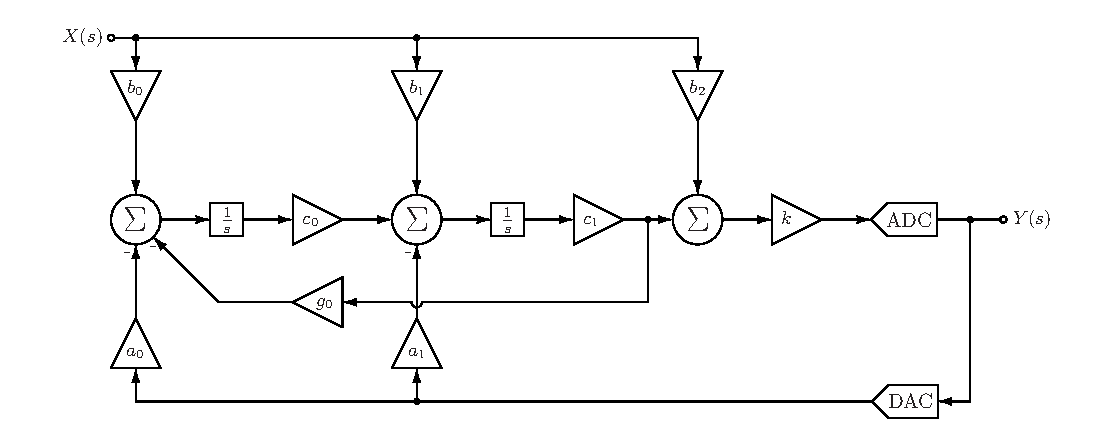
\includegraphics[width=\textwidth]{./final_figures/s_domain_sim_2.eps}
 \caption{2nd Order Block Diagram}
 \label{fig:2nd_order_block_diagram}
\end{figure}
%------------------------------------------
\vspace{-5mm}
\subsubsection*{Integrator Output 1 (scaled):}
%------------------------------------------
\begin{equation}\label{eq:2nd_order_node_1}
 \gamma _1(s)=\frac{c_0}{s}\bigl(b_0X(s)-a_0Y(s)-g_0\gamma _2\bigr)
\end{equation}

\subsubsection*{Integrator Output 2 (scaled):}
%------------------------------------------
\begin{equation}\label{eq:2nd_order_node_2}
\gamma _2(s)=\frac{c_1}{s}\bigl(\gamma _1(s)+b_1X(s)-a_1Y(s)\bigr)
\end{equation}

\subsubsection*{ADC Input (scaled):}
%------------------------------------------
\begin{equation}\label{eq:2nd_order_quantizer_input}
\gamma _3(s)=k\bigl(\gamma _2(s)+b_2X(s)\bigr) 
\end{equation}

\subsubsection*{Output:}
%------------------------------------------
\begin{equation}\label{eq:2nd_order_output_1}
 Y(s)=\gamma _3(s)+E(s)
\end{equation}

\vspace{2mm}
\noindent
Substituting \eqref{eq:2nd_order_node_1}-\eqref{eq:2nd_order_quantizer_input} into
\eqref{eq:2nd_order_output_1} and simplifying yields the following equation.
%------------------------------------------
\begin{equation}\label{eq:2nd_order_output_2}
Y=\frac{X\bigl(k s^2 b_2+k s b_1 c_1+k b_0 c_0 c_1+k b_2 c_0 c_1 g_0\bigr)+
E\bigl(s^2+c_0 c_1 g_0\bigr)}{s^2+k
s a_1 c_1+k a_0 c_0 c_1+c_0 c_1 g_0}
\end{equation}

\vspace{2mm}
\noindent
Substituting $k=1$ and $c_x=1$ into \eqref{eq:2nd_order_output_2} we arrive at the
following simplified expression.
%------------------------------------------
\begin{equation}\label{eq:2nd_order_output_3}
Y=X\biggl(\frac{s^2 b_2+s b_1+b_0+b_2 g_0}{s^2+s a_1+a_0+g_0}\biggr)+
E\biggl(\frac{s^2+g_0}{s^2+s a_1+a_0+g_0}\biggr)
\end{equation}

\vspace{2mm}
Comparing \eqref{eq:2nd_order_output_3} to \eqref{eq:STF_final} and \eqref{eq:NTF_final}
we can show the following set of equations.
%------------------------------------------
\begin{align*}
  F_0& = b_0+b_2 g_0& F_1& = b_1& F_2& = b_2 \\
 M_0& = a_0+g_0& M_1& = a_1& M_2& = 1 \\
  G_0& = g_0& G_1& = 0& G_2& = 1
\end{align*}
%------------------------------------------
Solving the above simultaneously for the coefficients in Figure
\ref{fig:2nd_order_block_diagram} in terms of the polynomial coefficients from
\eqref{eq:STF_final} and \eqref{eq:NTF_final} we arrive at the following.

\begin{align}\label{eq:2nd_order_solutions}
 a_0& = -G_0+M_0& a_1& = M_1& \\
 b_0& = F_0-F_2 G_0& b_1& = F_1& b_2& = F_2& \\
 g_0& = G_0&
\end{align}

\pagebreak

%% 3rd Order Block Diagram
 %%%%%%%%%%%%%%%%%%%%%%%%

\begin{center}
 \section*{3rd Order Block Diagram Reduction}
\end{center}

\begin{figure}[htb]
 \centering
 \includegraphics[width=\textwidth]{./final_figures/s_domain_sim_3.eps}
 \caption{3rd Order Block Diagram}
 \label{fig:3rd_order_block_diagram}
\end{figure}
%------------------------------------------
\vspace{-5mm}
\subsubsection*{Integrator Output 1 (scaled):}
%------------------------------------------
\begin{equation}\label{eq:3rd_order_node_1}
 \gamma _1(s)=\frac{c_0}{s}\bigl(b_0X(s)-a_0Y(s)\bigr)
\end{equation}

\subsubsection*{Integrator Output 2 (scaled):}
%------------------------------------------
\begin{equation}\label{eq:3rd_order_node_2}
\gamma _2(s)=\frac{c_1}{s}\bigl(\gamma _1(s)+b_1X(s)-a_1Y(s)-g_0\gamma _3(s)\bigr)
\end{equation}

\subsubsection*{Integrator Output 3 (scaled):}
%------------------------------------------
\begin{equation}\label{eq:3rd_order_node_3}
\gamma _3(s)=\frac{c_2}{s}\bigl(\gamma _2(s)+b_2X(s)-a_2Y(s)\bigr)
\end{equation}

\subsubsection*{ADC Input (scaled):}
%------------------------------------------
\begin{equation}\label{eq:3rd_order_quantizer_input}
\gamma _4(s)=k\bigl(\gamma _3(s)+b_3X(s)\bigr) 
\end{equation}

\subsubsection*{Output:}
%------------------------------------------
\begin{equation}\label{eq:3rd_order_output_1}
 Y(s)=\gamma _4(s)+E(s)
\end{equation}

\vspace{2mm}
\noindent
Substituting \eqref{eq:3rd_order_node_1}-\eqref{eq:3rd_order_quantizer_input} into
\eqref{eq:3rd_order_output_1} and simplifying yields the following equation.
%------------------------------------------
\begin{equation}\label{eq:3rd_order_output_2}
\begin{split}
Y&=E\biggl(\frac{s^3+s c_1 c_2 g_0}{s^3+k s^2 a_2 c_2+k a_0 c_0 c_1 c_2+s \bigl(k a_1 c_1
c_2+c_1 c_2
g_0\bigr)}\biggr)\\
&+X \biggl(\frac{k s^3 b_3+k s^2 b_2
c_2+k s b_1 c_1 c_2+k b_0 c_0 c_1 c_2+k s b_3
c_1 c_2 g_0}
{s^3+k s^2 a_2 c_2+k a_0 c_0 c_1 c_2+s \bigl(k a_1 c_1 c_2+c_1 c_2
g_0\bigr)}\biggr)
\end{split}
\end{equation}

\vspace{2mm}
\noindent
Substituting $k=1$ and $c_x=1$ into \eqref{eq:3rd_order_output_2} we arrive at the
following simplified expression.
%------------------------------------------
\begin{equation}\label{eq:3rd_order_output_3}
\begin{split}
Y&=E\Biggl(\frac{s^3+s g_0}{s^3+s^2
a_2+s \left(a_1+g_0\right)+a_0}\Biggr)\\
&+X\Biggl(\frac{s^3 b_3+s^2 b_2+s\left( b_1+
b_3g_0\right)+b_0}{s^3+s^2 a_2+s \left(a_1+g_0\right)+a_0}\Biggr)
\end{split}
\end{equation}

\vspace{2mm}
Comparing \eqref{eq:3rd_order_output_3} to \eqref{eq:STF_final} and \eqref{eq:NTF_final}
we can show the following set of equations.
%------------------------------------------
\begin{align*}
  F_0& = b_0& F_1& = b_1+b_3 g_0& F_2& = b_2& F_3 = b_3\\
 M_0& = a_0& M_1& = a_1+g_0& M_2& = a_2& M_3 = 1 \\
  G_0& = 0& G_1& = g_0& G_2& = 0& G_3 =1
\end{align*}
%------------------------------------------
Solving the above simultaneously for the coefficients in Figure
\ref{fig:3rd_order_block_diagram} in terms of the polynomial coefficients from
\eqref{eq:STF_final} and \eqref{eq:NTF_final} we arrive at the following.

\begin{align}\label{eq:3rd_order_solutions}
 a_0& = M_0& a_1& = M_1-G_1& a_2&=M_2\\
 b_0& = F_0& b_1& = F_1-F_3 G_1& b_2& = F_2& b_3& = F_3\\
 g_0& = G_1&
\end{align}

\pagebreak

%% 4th Order Block Diagram
 %%%%%%%%%%%%%%%%%%%%%%%%
 
 \begin{center}
 \section*{4th Order Block Diagram Reduction}
\end{center}

\begin{figure}[htb]
 \centering
 \includegraphics[width=\textwidth]{./final_figures/s_domain_sim_4.eps}
 \caption{4th Order Block Diagram}
 \label{fig:4th_order_block_diagram}
\end{figure}
%------------------------------------------
\vspace{-5mm}
\subsubsection*{Integrator Output 1 (scaled):}
%------------------------------------------
\begin{equation}\label{eq:4th_order_node_1}
 \gamma _1(s)=\frac{c_0}{s}\bigl(b_0X(s)-a_0Y(s)-g_0\gamma _2\bigr)
\end{equation}

\subsubsection*{Integrator Output 2 (scaled):}
%------------------------------------------
\begin{equation}\label{eq:4th_order_node_2}
\gamma _2(s)=\frac{c_1}{s}\bigl(\gamma _1(s)+b_1X(s)-a_1Y(s)\bigr)
\end{equation}

\subsubsection*{Integrator Output 3 (scaled):}
%------------------------------------------
\begin{equation}\label{eq:4th_order_node_3}
\gamma _3(s)=\frac{c_2}{s}\bigl(\gamma _2(s)+b_2X(s)-a_2Y(s)\bigr)
\end{equation}

\subsubsection*{Integrator Output 4 (scaled):}
%------------------------------------------
\begin{equation}\label{eq:4th_order_node_4}
\gamma _4(s)=\frac{c_3}{s}\bigl(\gamma _3(s)+b_3X(s)-a_3Y(s)\bigr)
\end{equation}

\subsubsection*{ADC Input (scaled):}
%------------------------------------------
\begin{equation}\label{eq:4th_order_quantizer_input}
\gamma _4(s)=k\bigl(\gamma _4(s)+b_4X(s)\bigr) 
\end{equation}

\subsubsection*{Output:}
%------------------------------------------
\begin{equation}\label{eq:4th_order_output_1}
 Y(s)=\gamma _4(s)+E(s)
\end{equation}

\vspace{2mm}
\noindent
Substituting \eqref{eq:4th_order_node_1}-\eqref{eq:4th_order_quantizer_input} into
\eqref{eq:4th_order_output_1} and simplifying yields the following equation.
%------------------------------------------
\begin{equation}\label{eq:4th_order_output_2}
\begin{split}
Y&=E\biggl(\frac{s^3+s c_1 c_2 g_0}{s^3+k s^2 a_2 c_2+k a_0 c_0 c_1 c_2+s \bigl(k a_1
c_1
c_2+c_1 c_2
g_0\bigr)}\biggr)\\
&+X \biggl(\frac{k s^3 b_3+k s^2 b_2
c_2+k s b_1 c_1 c_2+k b_0 c_0 c_1 c_2+k s b_3
c_1 c_2 g_0}
{s^3+k s^2 a_2 c_2+k a_0 c_0 c_1 c_2+s \bigl(k a_1 c_1 c_2+c_1 c_2
g_0\bigr)}\biggr)
\end{split}
\end{equation}

\vspace{2mm}
\noindent
Substituting $k=1$ and $c_x=1$ into \eqref{eq:3rd_order_output_2} we arrive at the
following simplified expression.
%------------------------------------------
% \begin{equation}\label{eq:3rd_order_output_3}
% \begin{split}Y=
% X\biggl(frac{(k s^4 b_4+k s^3 b_3 c_3+k s^2 b_2 c_2 c_3+k s b_1 c_1 c_2 c_3+k b_0
% c_0 c_1 c_2 c_3+k s^2 b_4 c_0 c_1 g_0+k s b_3 c_0 c_1 c_3
% g_0+k b_2 c_0 c_1 c_2 c_3 g_0+k s^2 b_4 c_2 c_3 g_1+k b_4 c_0 c_1 c_2 c_3 g_0
% g_1\right)\right/\right.\\
% \left.\left(s^4+k s^3 a_3 c_3+k a_0 c_0 c_1 c_2 c_3+k a_2 c_0 c_1 c_2 c_3 g_0+s \left(k
% a_1 c_1 c_2 c_3+k a_3 c_0 c_1 c_3 g_0\right)+c_0 c_1 c_2
% c_3 g_0 g_1+s^2 \left(k a_2 c_2 c_3+c_0 c_1 g_0+c_2 c_3 g_1\right)\right)\right)\\
% \end{split}
% \end{equation}

% \vspace{2mm}
% Comparing \eqref{eq:3rd_order_output_3} to \eqref{eq:STF_final} and \eqref{eq:NTF_final}
% we can show the following set of equations.
% %------------------------------------------
% \begin{align*}
%   F_0& = b_0& F_1& = b_1+b_3 g_0& F_2& = b_2& F_3 = b_3\\
%  M_0& = a_0& M_1& = a_1+g_0& M_2& = a_2& M_3 = 1 \\
%   G_0& = 0& G_1& = g_0& G_2& = 0& G_3 =1
% \end{align*}
% %------------------------------------------
% Solving the above simultaneously for the coefficients in Figure
% \ref{fig:3rd_order_block_diagram} in terms of the polynomial coefficients from
% \eqref{eq:STF_final} and \eqref{eq:NTF_final} we arrive at the following.
% 
% \begin{align}\label{eq:3rd_order_solutions}
%  a_0& = M_0& a_1& = M_1-G_1& a_2&=M_2\\
%  b_0& = F_0& b_1& = F_1-F_3 G_1& b_2& = F_2& b_3& = F_3\\
%  g_0& = G_1&
% \end{align}

\begin{equation*}
 z=3\bigl(1-x\bigr)^2
e^{\bigl(-x^{2}-\left(y+1\right)^{2}\bigr)}-10\Bigl(\frac{x}{5}-x^{3}-y^{5}\Bigr)e^{
\bigl(-x^{2}-y^{2}\bigr)}-\frac{1}{3}e^{\bigl(-\left(x+1\right)^{2}-y^{2}\bigr)}
\end{equation*}

 
\end{document}
